% !TEX root = ../notes.tex

\section{Basic concepts}
\subsection{A taste of "grammar"}

A data science student is attended to understand the \emph{Grammar of Data Science}. We are going to learn the core data manipulations, so no matter what is the backend. \texttt{SQL, pandas} and \texttt{R}(with \texttt{dplyr}) all share the same\emph{ grammar}. 
For sure having some backgrounds in SQL concepts is a good thing because, as it is very common, people love to make examples with it. Here is a brief refresh of some definitions and concepts that are essential and we need to be aware of.

Let's start with two key concepts that \emph{Structured data} requires:

\begin{itemize}
  \item {\bf Data model}: a collection of concepts for describing data.
  \item {\bf Schema}: a description of a particular collection of data, using a given data model.
\end{itemize}

The most common and ubiquitous approach to manage data is the \emph{Relational model} (\href{https://en.wikipedia.org/wiki/Edgar\_F.\_Codd}{E. F., Ted Codd}). It can handle most of the data, so most of it is "reduced" to this model. To have an idea, a counter example is the facebook-like data which requires {\bf graph model}. 

The \emph{Relational model} is composed by relations. A \emph{relation} is made up two parts:

 \begin{enumerate}
 \item The {\bf Schema} specifies name of relation, plus name and type of each column. \\ For example, \verb+Students(sid: string, name:string, age:integer)+
  \item The {\bf Instance}, {\it i.e.} the data at a given time. \\
  Definitions:
  \begin{itemize}
   \item {\bf Cardinality} is the number of rows (= number of items)
   \item {\bf Degree} or {\bf Arity} is the number of fields ( = number of attributes)
  \end{itemize}
 \end{enumerate}

\subsection*{Database vocabulary}

Here follows a list of basic words and operations that should be kept in mind when we talk about \emph{Databases}.

 \begin{itemize}
  \item A \texttt{JOIN} is a mean to combine tables based on shared attributes (most of the time some \texttt{IDs}). Despite its apparent simplicity beware of the many ways to compute a \texttt{JOIN} and check what is the default \texttt{JOIN} of a language before using it. Every different \texttt{JOIN} operation has implications on the resulting relation. The Figure \ref{join_SQL} summarises these possibilities.
  \item \emph{Aggregation}, \emph{reduction}, and \texttt{groupby} are the actions of reducing data with a common operation (\texttt{sum}, \texttt{count}, \texttt{average}, ...) to summarize them. Remember that you always need to specify the \emph{attribute} you are going to perform the \emph{aggregation} on.
 \end{itemize}
  
\subsection{Our tools}

During this course and, likely, in your future, to handle data you are going to use a \emph{'magic'} \texttt{Python}'s tool that has a black and white coat, with black fur around its eyes: \texttt{pandas}. 

The basic ingredients of our beloved \texttt{pandas}:

\begin{itemize}
 \item \texttt{Series} are a name, ordered dictionary
\begin{itemize}
 \item keys are indexes
 \item built on \texttt{numpy.ndarray} (so values can be any \texttt{Numpy} data type)
\end{itemize} 
\end{itemize}


\begin{itemize} 
 \item \texttt{DataFrame} is a table with named column
  \begin{itemize}
  \item the columns are series
  \item it is indeed a dictionary with (columnName $\rightarrow$ series)
  \end{itemize}  
\end{itemize}

Learn how to use \href{https://github.com/ADAEPFL/Labs/tree/master/02\%20-\%20Intro\%20to\%20Pandas}{\texttt{pandas}} and discover the beauty of \href{https://github.com/ADAEPFL/Labs/tree/master/01\%20-\%20Intro\%20to\%20Tools}{\texttt{IPython Notebooks}}.

\begin{figure}%---------------FIG--------------
 \centering
 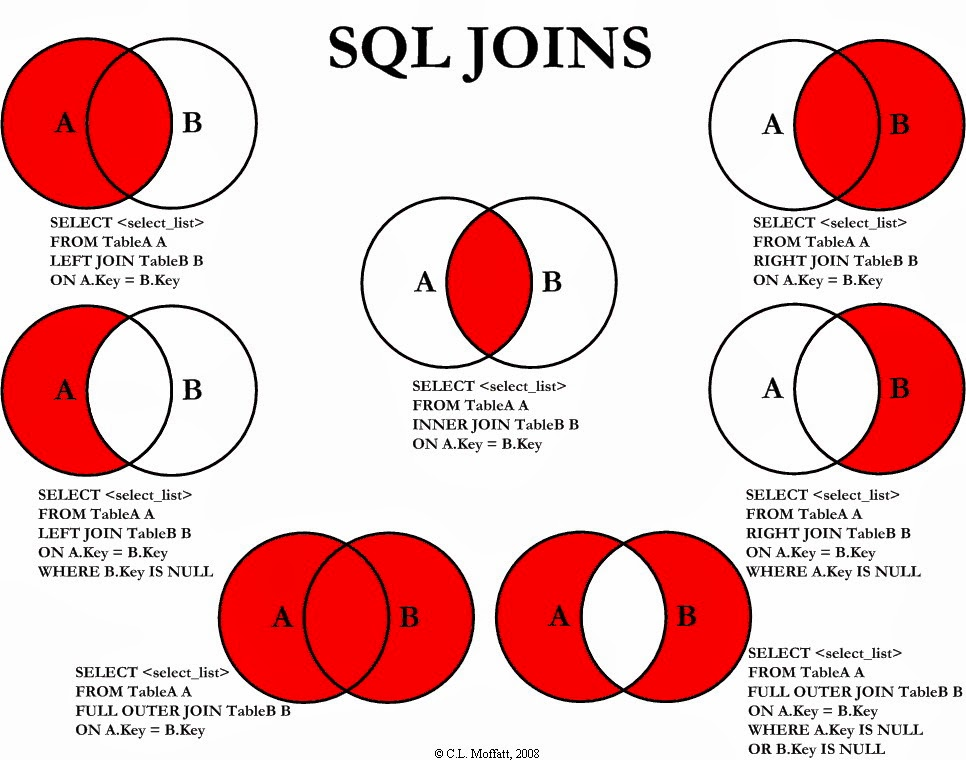
\includegraphics[width=12cm]{./img/02/SQL_joins}
 \caption{\label{join_SQL} Different ways to join two tables and the related SQL command.}
\end{figure}


\subsection{Panda vs SQL}

Panda is built to allow easy and fast \textbf{data exploration} and not to be a database manager, as SQL is. Thus there are benefits and drawbacks of using it.


\begin{center} %---------------TAB--------------
\begin{tabular} {| l | l |}
\hline
\bf Pros & \bf Cons \\ \hline
Lightweight \& fast & Tables stored directly in memory \\
Great expressiveness (combine SQL + Python) & No post-load indexing functionality\\
Easy plot for data visualization (e.g. Matplotlib) & No transactions, journalings\\ 
& Large, complex joins are slower \\ \hline
\end{tabular}
\end{center}

\subsection{OnLine Analytical Processing (OLAP cubes)}

OLAP tools enable users to analyze multidimensional data interactively from multiple perspectives. Conceptually, it is like an n-dimensional spreadsheet (a cube) on which we can apply various operations to take decisions.

OLAP cubes are another way to see data tables and are constructed based on them, as shows FIG \ref{OLAP_cubes}.

\begin{figure}[H]%---------------FIG--------------
 \centering
 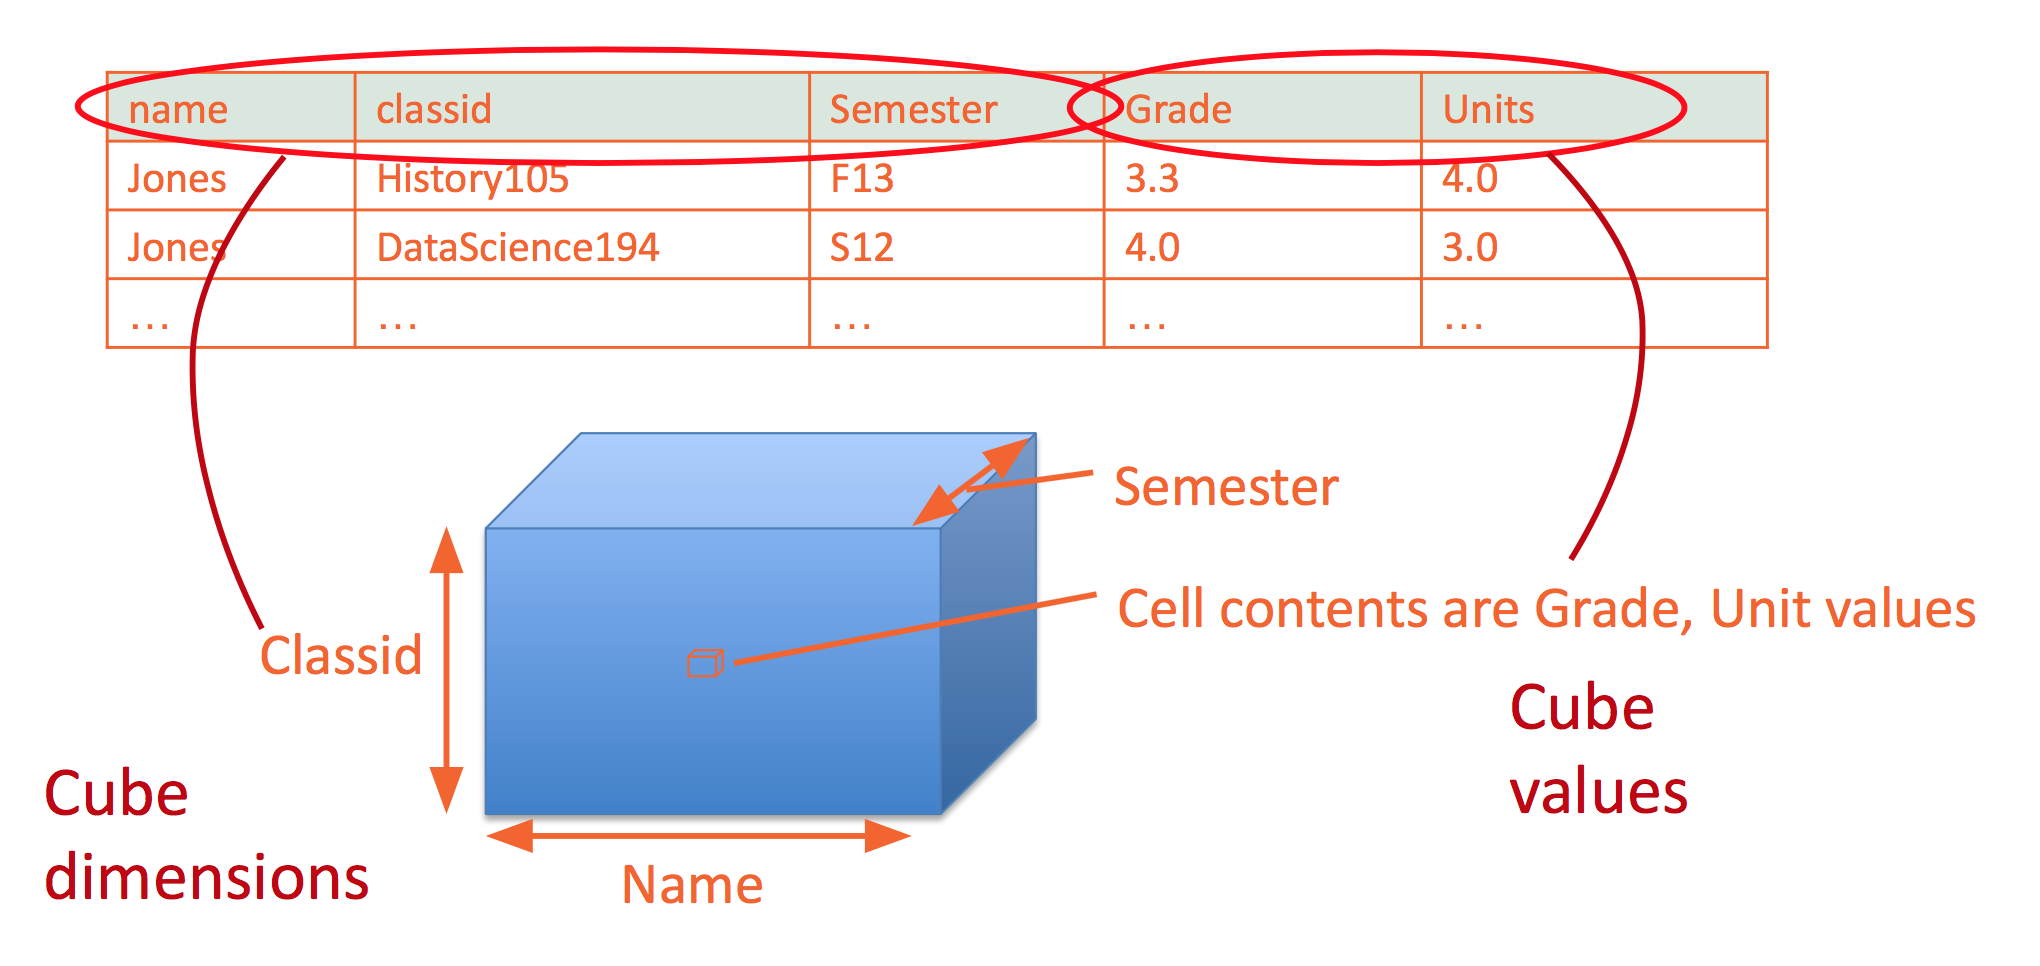
\includegraphics[width=12cm]{./img/02/OLAP_cube}
 \caption{\label{OLAP_cubes} Construction of an OLAP cube from a table.}
\end{figure}

Operations on OLAP cubes are the following and are illustrated on FIG \ref{OLAP_operations}
\begin{itemize}
	\item \textbf{Slicing} fixes one or more variable
	\item \textbf{Dicing} selects a range of one or more variable
	\item \textbf{Drilling up/down} change levels of a hierarchically indexed variable, i.e. "zoom" on a variable and see the subcategories it contains.
	\item \textbf{Pivoting} change the point of view of the cube. Swap an aggregated variable and a detailed one.
\end{itemize}

\begin{figure} [h] %----------- SubGraph ---------------------
\centerline{
\subfigure[Slincing\label{olap_slicing}] {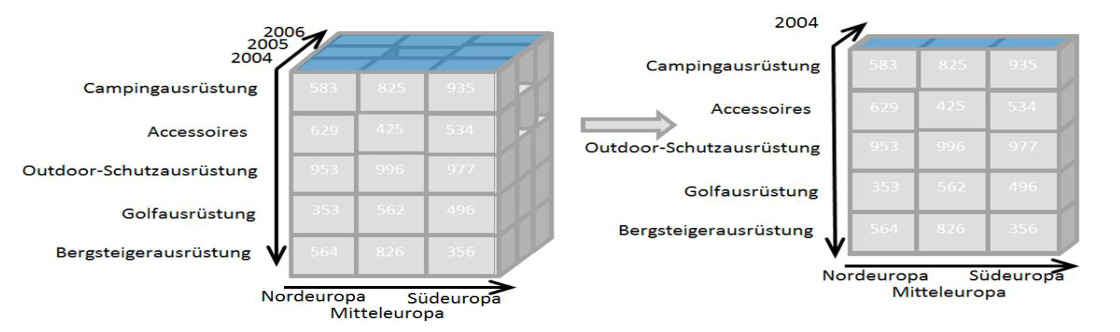
\includegraphics[width=7cm]{img/02/Slicing} }
\subfigure[Dicing\label{olap_dicing}] {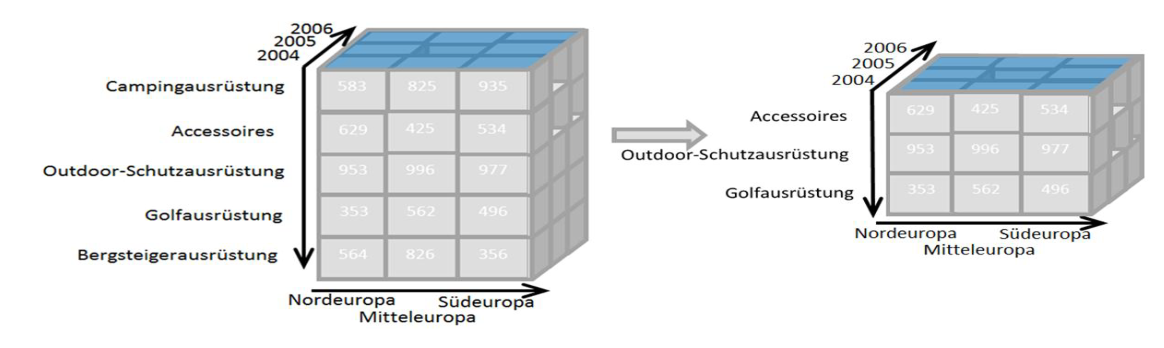
\includegraphics[width=7cm]{img/02/Dicing} } 
}
\centerline{
\subfigure[Driling up/down\label{olap_driling}] {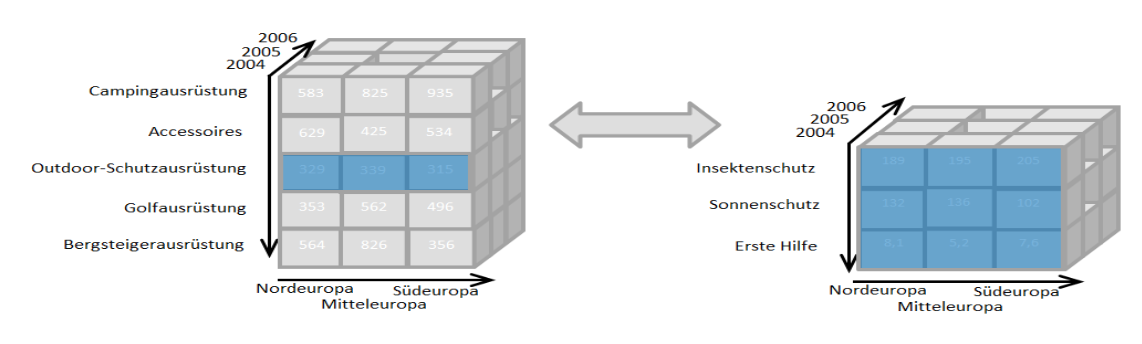
\includegraphics[width=7cm]{img/02/Drilling_up_down} }
\subfigure[Pivoting\label{olap_pivoting}] {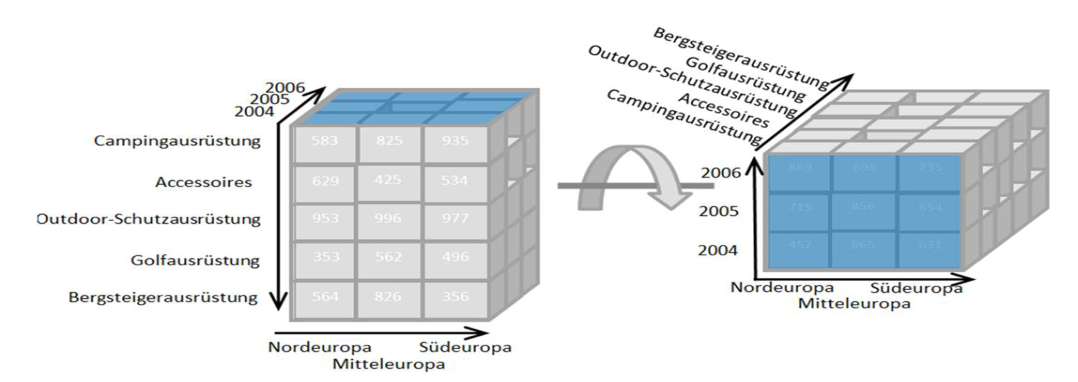
\includegraphics[width=7cm]{img/02/Pivoting} } 
}
\caption{\label{OLAP_operations} Operations on OLAP cubes} 
\end{figure}

\begin{center} %---------------TAB--------------
\begin{tabular} {| l | l |}
\hline
\bf Pros & \bf Cons \\ \hline
& \\
\parbox[t][][t]{7cm}{The main advantage of OLAP cubes is that they are \textbf{conceptually simpler} to understand by a non-scientist person, e.g. a business man who has to take day-to-day decisions based on company's data. Aggregations are limited but cover the main common cases that we can encounter.
}&
\parbox[t][][t]{7cm}{Because of the "on-line" behaviour of this approach, all types of aggregation must be pre-calculated among all combinations of axes which is very \textbf{expensive in memory and in time} (when updating the data)}\\
& \\
\hline
\end{tabular}
\end{center}
